\chapter{Stage}
\label{chap:stage}


\section{Introduzione al progetto}
\label{sec:introstage}
Lo stage ha avuto una durata di 3 mesi, dal 07/10/2019 al 07/01/2020 presso la sede milanese di SIA S.p.A in Via Privata Francesco Gonin 36. \\

Come accennato nell' \hyperlink{introduzione}{introduzione}, il contenuto dello stage verte principalmente sullo sviluppo di una \textit{Web Application}, commissionata dall'azienda SIA S.p.A all'azienda Innovery S.p.A.
Il progetto in questione ha come obiettivo principale l'ottimizzazione del processo di \textit{onboarding} di flussi logici che devono essere condivisi tra Business Partners e che devono passare attraverso un \gls{systemintegrator}, \textit{IBM® Sterling B2B Integrator}. \\

\subsection{IBM® Sterling B2B Integrator}
IBM® Sterling B2B Integrator è un motore di transazione che esegue \textit{Business Process}, supporta lo scambio di messaggi elettronici ad alto volume, l'instradamento complesso, la traduzione, il trasferimento gestito di file (\gls{MFT}) e l'integrazione flessibile con più sistemi interni e partner commerciali esterni. Include strumenti di gestione visiva per la configurazione e la visibilità dei flussi di lavoro, le attività del sistema e dei partner commerciali, le mappe di traduzione e l'implementazione dei \textit{Business Process}. Funziona con centinaia di protocolli aziendali e standard di comunicazione emergenti \cite{ibmsterling}.

Tra i componenti principali di questo complesso sistema abbiamo:
\begin{itemize}
    \item \textit{Business Process}: un flusso di attività ordinato e orientato al raggiungimento degli obiettivi aziendali. Ogni \textit{Business Process} è definito da un unico documento \gls{BPML}.
    \item \textit{Services}: una risorsa che è possibile configurare per svolgere un'attività. 
    \item \textit{Adapters}: casi speciali di \textit{Services} che interagiscono con sistemi esterni o che archiviano o gestiscono dati di stato al di fuori del contesto del flusso di lavoro.
\end{itemize}



\clearpage

\begin{figure}
\begin{center}
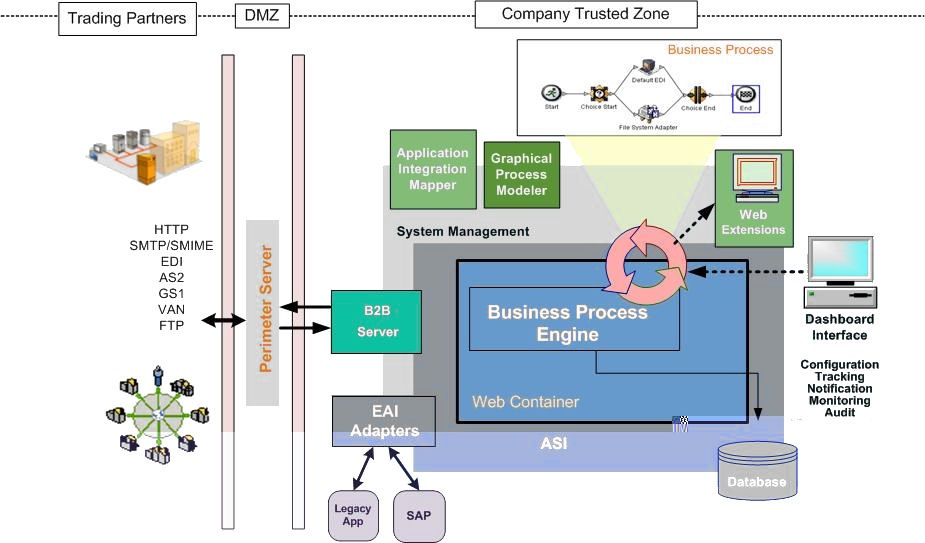
\includegraphics[width=1.0\columnwidth]{images/ibmarchitecture.jpg}
\end{center}
\caption{Architettura software IBM® Sterling B2B Integrator}
\label{fig:archi_sterling}
\end{figure}


\subsection{Architettura già esistente}
L'azienda SIA S.p.a presenta un'infrastruttura di tipo \textit{cluster}, un insieme di computer connessi tra loro tramite una rete telematica. Scopo del \textit{cluster} è distribuire un'elaborazione molto complessa tra i vari computer, aumentando la potenza di calcolo del sistema e garantendo una maggiore disponibilità di servizio, a prezzo di un maggior costo e complessità di gestione dell'infrastruttura \cite{cluster}. Come si evince dalla figura \ref{fig:archi_sia} sono presenti due macchine sulle quali è installato IBM® Sterling B2B Integrator, ambedue i nodi condividono lo stesso database e inoltre si scambiano informazioni riguardanti il carico, lo stato dell'applicazione e del nodo. L'architettura presenta inoltre i seguenti componenti per aumentare la sicurezza dell'infrastruttura:
\begin{itemize}
    \item \textit{Firewall}: hardware e software per controllare il traffico in ingresso/uscita di una rete fidata rispetto a reti non sicure
    \item \textit{Application Proxy}: interfaccia di comunicazione in una rete per monitorare il traffico fra applicazioni
    \item \textit{DMZ}: zona demilitarizzata, indica una rete di computer, che funge tra due reti da zona cuscinetto con un proprio indirizzo IP e le delimita mediante regole di accesso rigide
\end{itemize}
Per mantenere l'integrità dell'architettura, la \textit{Web Application} verrà installata su entrambi i nodi dove è installato il prodotto IBM® Sterling B2B Integrator, sarà però attivata solo su uno dei due. (In \ref{fig:archi_sia} IBM® Sterling B2B Integrator è abbreviato con SFG)



\clearpage

\begin{figure}
\begin{center}
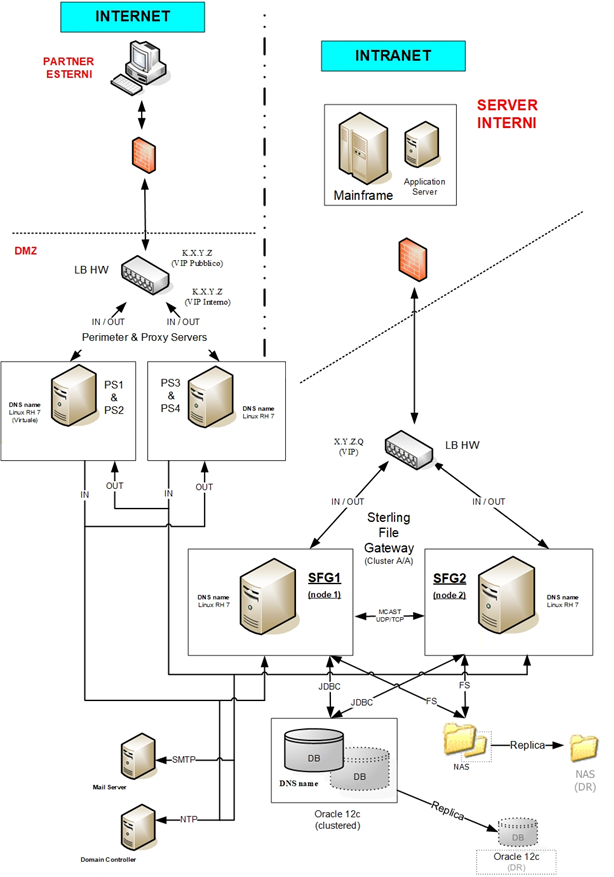
\includegraphics[width=0.9\columnwidth]{images/siaarch.png}
\end{center}
\caption{Architettura installata in SIA S.p.A}
\label{fig:archi_sia}
\end{figure}

\clearpage


\subsection{Processo di onboarding flussi}
\label{subsec:onboarding}
Per processo di \textit{onboarding} di flussi logici, si intende la registrazione di informazioni utili per la gestione e l'implementazione di regole di instradamento per i file che passano attraverso il prodotto IBM® Sterling B2B Integrator.
Le informazioni necessarie possono essere suddivise in 3 categorie: informazioni sistemistiche, operazionali e metadati.

Per informazioni sistemistiche intendiamo tutte quelle informazioni riguardanti:
\begin{itemize}
    \item \Gls{ip}
    \item Porta \gls{tcpip}
    \item Protocollo utilizzato
\end{itemize}
Queste informazioni servono per poter definire \textit{"come"} un \gls{businesspartner} ha intenzione di interfacciarsi con il \gls{systemintegrator}, con lo scopo di inviare e/o ricevere file. \\
Le informazioni operazionali rappresentano informazioni riguardanti alle operazioni che possono essere effettuate sul file prima di essere consegnato al \gls{businesspartner} destinatario. Tra le operazioni possibili abbiamo:
\begin{itemize}
    \item Ridenominazione: rinomina il nome del file.
    \item Backup: salva una copia del file.
    \item Compressione: effettua una riduzione delle dimensioni del file attraverso uno specifico algoritmo. 
    \item Decompressione: riporta un file precedentemente compresso alle condizioni iniziali.
    \item Cifratura: applica un algoritmo di cifratura specifico per rendere il contenuto del file incomprensibile.
    \item Decifrazione: applica un algoritmo di cifratura specifico per rendere il contenuto del file leggibile.
    \item Codifica \gls{charset}: converte i caratteri del \gls{charset} iniziale in caratteri di un altro \gls{charset}.
\end{itemize}

Per poter instradare correttamente un file i metadati necessari sono:  \gls{businesspartner} mittente, destinatario e regola che identifica univocamente il file. La regola richiesta è nella nomenclatura del file da gestire, quest'ultima dovrà avere all'inizio del nome del file la seguente sintassi:
\begin{center} \textbf{SERVICE.ABI.FILETYPE.}[Nome file originale]\end{center}

I 3 identificatori sono separati da un punto, hanno una lunghezza prefissata e vengono concordati in fase di analisi con i \glspl{businesspartner}. Il primo identificatore indica il servizio di cui il file fa parte, il secondo denota il \gls{codiceabi} del mittente mentre il terzo il tipo file. Nello specifico il terzo elemento denota il formato e la logica del contenuto del file.


Come accennato precedentemente, all'arrivo di un file, il prodotto  IBM®Sterling B2B Integrator utilizzerà queste informazioni per poter correttamente instradare il file verso il destinatario.








% L'implementazione di questa applicazione si pone come traguardo il permettere al team \textit{Sistemisti File Transfer}, team che lavora all'interno dell'azienda SIA S.p.A. di ottimizzare il loro \textit{'day-to-day work'} nel implementare le varie regole per quanto riguarda il transito dei file attraverso le loro macchine. Perciò l'applicazione oltre ad essere integrata con l'implementazione architetturale presente, dovrà anche possedere una User Interface, facile ed intuibile che permetta al Team \textit{Sistemisti File Transfer} di essere veloci e flessibili con le richieste dei vari progetti. \\



\section{Obiettivi}
\label{sec:obiettivi}


\subsection{Obiettivi personali}
\label{subsec:obiettivipersonali}

Gli obiettivi prefissati inizialmente sono stati :

\begin{itemize}
    \item Approfondimento delle conoscenze nell'ambito sviluppo Web, in particolar modo 
    dello sviluppo \gls{FULL-STACK}, lavorando dunque sia sulla parte riguardante il \textit{back-end} e quella riguardante il \textit{front-end} (cfr. \ref{sec:inqgenerale}).
    
    \item Collaborare con un team di sviluppo con esperienza, che applichi le \gls{bestpractices} per lo sviluppo e la metodologia \textit{agile} (cfr. \ref{sec:pianodilavoro}).
    
    \item Acquisire competenze nello sviluppo di software che ha lo scopo di integrarsi con altre soluzioni già esistenti.
    
    \item Approfondimento delle conoscenze nell'ambito bancario/finanziario, per quanto riguarda pagamenti, carte, banche..
\end{itemize}

\subsection{Obiettivi dell'azienda}
\label{subsec:obiettiviazienda}
Gli obiettivi dell'azienda SIA S.p.A. per questo progetto sono stati:

\begin{itemize}
    \item Ottimizzare il processo \textit{onboarding} di flussi logici che devono essere condivisi tra \glspl{businesspartner} e che devono passare attraverso il \gls{systemintegrator} \textit{IBM® Sterling B2B Integrator}.
    \item Aumentare il livello di personalizzazione dei propri prodotti.
    \item Mantenere l'architettura già esistente intatta.
\end{itemize}



\section{Piano di lavoro}
\label{sec:pianodilavoro}

Per il modello di sviluppo si è scelto di utilizzare il paradigma \textit{agile}, esso definisce principalmente quattro fondamenti, ovvero: \cite{agile} \cite{agilemanifesto}

\begin{itemize}
    \item Le persone e le interazioni sono più importanti dei processi e degli strumenti;
    \item È più importante avere software funzionante che documentazione;
    \item Bisogna collaborare con i clienti oltre che rispettare il contratto;
    \item Bisogna essere pronti a rispondere ai cambiamenti oltre che aderire alla pianificazione;
\end{itemize}


In particolare la metodologia \textit{agile} utilizzata in questo contesto è stata \textit{Scrum}. Si tratta di \gls{framework} per la gestione del ciclo di sviluppo del software, iterativo ed incrementale, concepito per gestire progetti e prodotti software o applicazioni di sviluppo. \textit{Scrum} struttura il proprio sviluppo in cicli chiamati \textit{Sprint} che durano da una a quattro settimane, al termine dei quali il team di sviluppo rilascia funzionalità immediatamente testabili.

\clearpage
I cicli sono \textit{timeboxed}, il che significa che hanno durata fissa nel tempo, non possono essere estesi e terminano anche se il lavoro non è stato ultimato. All’inizio di ogni \textit{Sprint}, durante un evento chiamato \textit{Sprint Planning}, il team seleziona i propri task da una lista di attività priorizzate \textit{Product Backlog} e si impegna a completare tutte le attività selezionate entro il termine dello \textit{Sprint}. Il fine ultimo non è completare il maggior numero di attività possibile, ma produrre incrementi di software utilizzabili, raggiungendo lo \textit{Sprint Goal} ovvero l’obiettivo che si desidera ottenere durante l’iterazione.\\
Il team si confronta quotidianamente mediante il \textit{Daily Scrum Meeting}, una riunione di pochi minuti con lo scopo di fare un recap degli obiettivi  del giorno. Al termine di ogni \textit{Sprint} vi sono due incontri fondamentali: lo \textit{Sprint Review} e il \textit{Retrospective Meeting}.
Il primo è un meeting informale in cui il team valida il lavoro svolto, il secondo che in genere è svolto al termine del primo, serve al team per riflettere sullo Sprint appena concluso \cite{scruminfo}.\\\\


\begin{figure}
\begin{center}
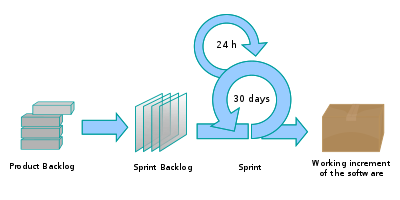
\includegraphics[width=1.0\columnwidth]{images/Scrum_process.png}
\end{center}
\caption{Modello del ciclo di sviluppo software Scrum}
\label{fig:scrum}
\end{figure}


\clearpage


\subsection{Diagramma di Gantt}
Di seguito viene riportato il \gls{diagrammagantt} che indica la suddivisione del lavoro durante tutto il periodo di stage. Il seguente diagramma è stato tracciato con il tutor aziendale Nicola Frongia, e condiviso con il team di sviluppo.\\ 



\begin{figure}
\begin{center}
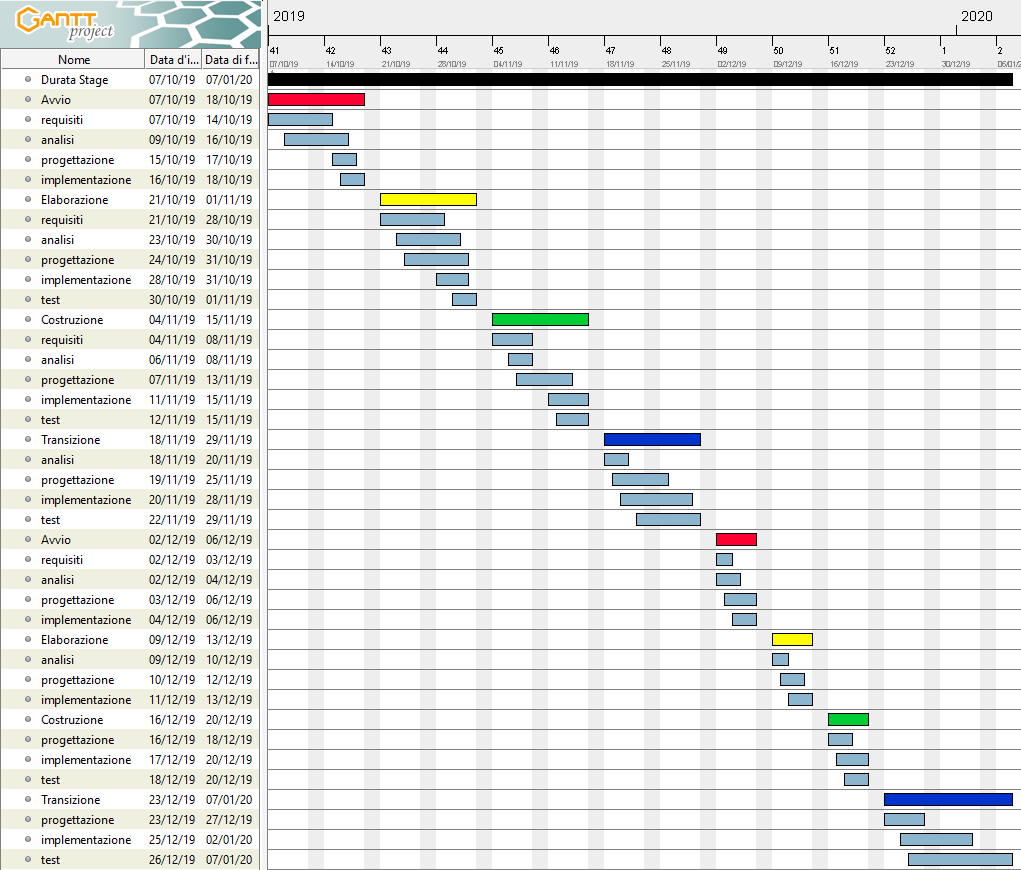
\includegraphics[width=1.0\columnwidth]{images/ganttstoianov.png}
\end{center}
\caption{Diagramma di Gantt per pianificazione dello stage}
\label{fig:gantt}
\end{figure}




